\section{Key Idea}
\label{sec:keyidea}

The key idea of \verb|OFF| file is storing the 3-D object's informations, including vertices, faces, and edges.

For vertice, the x, y, z coordinates will be recorded.
For face, the indexes of vertices for a face will be recorded.
For edge, that should be ignored in this dataset.

To represent a 3-D object, there are vertices and faces needed.
For example, if we need to represent a cube and assume its size is $ 2 \times 2 \times 2$ with its center located at point $(0,0,0)$.

\section{Example}
\label{sec:example}

There are some examples.

The first example is a triangluar prism.
The following codes is the OFF file, and the fig.\ref{fig:test2} is preview of item.

\begin{lstlisting}[caption=Demo of script]
OFF
6 5 0
0 0 0
0 1 0
1 0 0
0 0 1
0 1 1
1 0 1
3 1 0 2
3 4 3 5
4 0 1 4 3
4 0 2 5 3
4 1 2 5 4
\end{lstlisting}

The second and thrid examples are a bed(id:0572) and a table(id:0440),
and the fig.\ref{fig:bed:0572} and fig.\ref{fig:table:0440} is the preview of
models.
\begin{figure}
    \centering
    \subfigure[Example in test script]{
        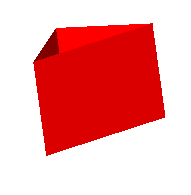
\includegraphics[width=0.3\linewidth]{/img/deep-learning/test2}
        \label{fig:test2}
    }
    \subfigure[Example, bed 0572]{\
        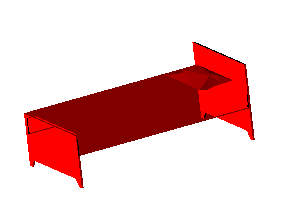
\includegraphics[width=0.3\linewidth]{/img/deep-learning/bed_0572}
        \label{fig:bed:0572}
    }
    \subfigure[Example, table 0440]{
        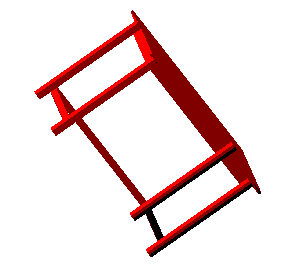
\includegraphics[width=0.3\linewidth]{/img/deep-learning/table_0440}
        \label{fig:table:0440}
    }
    \caption{Examples of dataset's data}
    \label{fig:eg}
\end{figure}

\section{hOff display}
\label{sec:hoff}

The \verb|hOff-display| is a OpenGL based tool to used to preview the model in
Princeton ModelNet dataset. It is open source and the
\href{https://github.com/Qinka/hOff}{repo} is available on GitHub with GPLv3 License. It is also available on \href{http://hackage.haskell.org/package/hOff-display}{Hackage}.

